
 
\section{Expressiveness Theory for Transformers with Chain of Thought(CoT)}\label{sec:main_result}

In this section, we study the expressiveness of transformers with CoT from a theoretical perspective. 

\subsection{Finite Precision Modeling}\label{subsec:finite_precision}

In practice, training and inference of transformers are typically done with 16- or 32-bit floating point numbers. Thus in this paper, we mainly focus on the computation model of \emph{constant-precision} transformers, where the output of each arithmetic operation is rounded to the closest  floating point number representable by a fixed number of digits following IEEE 754 standard (\Cref{defi:rounding}), thus avoiding the unrealistic infinite precision assumption made by prior works~\citep{perez2019turing, dehghani2018universal}.


Below we give a formal definition of the \emph{floating-point number} and \emph{rounding} operation. Recall  $\phi(a) = \sum_{i=1}^k 2^{k-i}a_i$ denote the value of binary number represented by $a\in \{0,1\}^k$ for any $k\in\mathbb{N}^+$. 



\begin{definition}[Floating-point Representation]
Let $e$ be the number of bits for exponents and $s$ be the number of bits for significand.  A $(e+2s+1)$-bit binary string $a = (a_1, a_2, \ldots a_{e+2s+1})\in \{0,1\}^{e+2s+1}$ is a \emph{floating-point} binary representation of number $\phi_{e,s}(a)\triangleq \sign(a)\cdot 2^{\exponent(a)} \cdot \significand(a)$ with $e$-bit exponent and $2s$-precision, where the sign is $\sign(a)\triangleq 2a_1-1$, the significand is $\significand(a)\triangleq 2^{-s}\phi(a_{2:2s+1})$, and the exponent is $\exponent(a)\triangleq \phi(a_{2s+2:2s+e+1})-2^{\max(0,e-1)}$. We further use $\Floating_{e,s}$ to denote all the floating numbers representable using $e$-bit exponent and $2s$-bit precision (significand), that is, $\Floating_{e,s}\triangleq \{ S\cdot 2^{-s +E} \mid -2^{2s}+1\le S\le 2^{2s}-1, -2^{\max(0,e-1)}\le E\le 2^e -1 -2^{\max(0,e-1)}, E,S\in\mathbb{N} \}$. We define $B_{e,s}\triangleq \max \Floating_{e,s}$.
\end{definition}

We also use $\psi_{e,s}:\Floating_{e,s}\to \{0,1\}^{e+2s+1}$ to denote the inverse of $\phi_{e,s}$. We note that when the number of exponent bits is larger than $0$, there are multiple ways to represent a number in $\Floating_{e,s}$ by a binary string and we assign $\psi_{e,s}(x)$ as the string $a\in\{0,1\}^{e+2s+1}$ with the smallest $\abs{\exponent(a)}$, which is unique for all non-zero numbers. For $0$ we additionally set $\sign(\psi_{e,s}(0))=1$. 

\begin{definition}[Correct Rounding]\label{defi:rounding} 
	 For any $x\in \mathbb{R}$ and any closed subset of $\mathbb{R}$ containing $0$, $\Floating$, we define \emph{correct rounding} $\round(x,\Floating)$ as the closest number to $x$ in $\Floating$. We break the tie by picking the one with a smaller absolute value. 
 
 In particular, we denote the rounding operation with $e$-bit exponent, $2s$-bit precision by $\round_{e,s}(\cdot)\triangleq \round(\cdot,\Floating_{e,s})$, which is also denoted by $\rdes{\cdot}$ for convenience. We extend the definition of $\round$ and $\round_{e,s}$ to vector inputs by rounding coordinate-wisely. 
\end{definition} 

Our notion of floating-point number simplifies the IEEE 754 Standard for Floating-point Arithmetic~\citep{ieee754_2008} by removing $\infty$ and $-\infty$. When overflow happens, we always round the output to the (negative) largest representable number in $\Floating_{e,s}$. For unary functions like $\exp(\cdot)$ and binary functions including addition, subtraction, multiplication, and division, we simply define their rounded version by rounding their outputs. Whenever division by $0$ happens, we treat it as the model outputs the wrong result.

 Next, we define finite-precision summation over more two numbers by decomposing it as a chain of rounded binary addition in a fixed order. \footnote{Technically speaking, instead of a chain, the summation could also proceed like a tree. This is a more complicated case and we leave it for future work. }

\begin{definition}[Summation with Iterative Rounding] For any $s,n\in\mathbb{N}^+$ and vector $x\in\mathbb{R}^n$, we define \emph{summation with iterative rounding to $e$ bit exponent and $2s$-bit precision} as $\sumes:\cup_{n\in\mathbb{N}^+}(\Floating_{e,s})^n\to \Floating_{e,s}$\ , where for any $n\in\mathbb{N}^+$ and $x\in\mathbb{R}^n$, $$\sumes(x)\triangleq \rdes{\rdes{\rdes{\rdes{x_1+x_2}+x_3}+\cdots x_{n-1}}+x_n}.$$

We further define the following operations:
\begin{itemize}
	\item Finite-precision inner product: $\inner{x}{y}_{e,s}\triangleq \sumes(x\odot y)$;
	\item Finite-precision matrix product: $(A\times_{e,s} B)_{i,j} \triangleq \inner{(A_{i,:})^\top}{B_{:,j}}_{e,s}$\ ;
	\item Finite-precision softmax: $\softmax_{e,s}(x)\triangleq \rdes{\rdes{\exp(x)}/\sumes(\rdes{\exp(x)})}$\ .
\end{itemize}
\end{definition}

%%%%% zhiyuan: save for now
%We note that the summation order is not specified by the algorithm and is often implementation-dependent in practice. Moreover, the summation order could even be non-deterministic due to parallelization, which makes the result non-deterministic for finite-precision numbers.~\citep{defour2014increasing,chou2020deterministic}. \zhiyuan{add discussion} 

Finally,  a finite-precision transformer can be defined by replacing all the infinite-precision operations by their finite-precision counterparts listed above. (See details in \Cref{alg:defi_transformer_finite_precision}). We postpone the details of the finite-precision version of individual transformer layers into \Cref{appsec:finite_precision}. 



 
\subsection{$\Cot$: Complexity Class for Constant-depth Transformers with CoT}


In this subsection, we define the complexity class consisting of all the problems that can be solved by some decoder-only transformers with $\Cot$ with finite precision.  

\begin{definition}[$\Cot$]\label{defi:complexity_cot}
	Given a finite vocabulary $\gV$ and four functions $T(n),d(n),s(n),e(n)$, informally, $\Cot[T(n)][d(n)][s(n)][e(n)]$ is the family of problems solvable by a transformer with a constant depth, $s(n)$ bits of precision, $e(n)$ bits of exponent, embedding size $d(n)$ and $T(n)$ steps of CoT. Formally, we say a problem  $\gL:\cup_{n\in\mathbb{N}^+}\gV^n\to \{0,1\}$ is in $\Cot[T(n)][d(n)][s(n)][e(n)]$ iff there is an integer $L$ and three functions $T'(n) = O(T(n)), d'(n) = O(d(n)), s'(n) = O(s(n))$, $e'(n) = O(e(n))$, such that for every positive integer $n$, there is a $L$-layer decoder-only transformer, denoted by $\transformer_{\theta_n}$ with embedding size $d'(n)$, $2s'(n)$ bits of precision, and $e'(n)$ bits of exponent, that can output $\gL(x)$ given any input $x$ in $\gV^n$, using $T'(n)$ steps of chain of thought. Mathematically, it means 
	\begin{align}
	\transformer_{\theta_n}^{1+ T'(n)}(x) = \gL(x)	, \quad \forall x \in \gV^n.
	\end{align}
We also extend the definition of $\Cot$ to a class of function instead of a single function. For example, $\Cot[T(n)][\poly(n)][s(n)][e(n)]\triangleq \cup_{k\in\mathbb{N}^+} \Cot[T(n)][n^k][s(n)][e(n)]$.
\end{definition}

\begin{definition}[$\T$] We define $\T[d(n)][s(n)][e(n)]\triangleq \Cot[0][d(n)][s(n)][e(n)]$ as the problems that a constant-depth, constant-precision decoder-only transformer can solve with $O(s(n))$ bits of precision, $O(e(n))$ bits of exponent, $O(d(n))$ embedding size and without CoT (or with only $0$ step of CoT).
\end{definition}

By definition, $\Cot[T(n)][d(n)][s(n)][e(n)]$ is monotone in all $T(n), d(n), s(n), e(n)$, \emph{e.g.}, $\Cot[T'(n)][d(n)][s(n)][e(n)]\subseteq \Cot[T(n)][d(n)][s(n)][e(n)]$ if $T'(n)\le T(n)$ for all $n\in \mathbb{N}$. In particular, we have $\T[d(n)][s(n)][e(n)] \triangleq \Cot[0][d(n)][s(n)][e(n)] \subseteq \Cot[T(n)][d(n)][s(n)][e(n)]$.


Note the above-defined complexity class $\Cot$ is non-uniform, that is, it allows a different program for every input size. This is in contrast to previous works~\citep{perez2019turing, perez2021attention,yao2021self,weiss2021thinking,chiang2023tighter,hao2022formal,merrill2023logic,merrill2022saturated} which focus on the uniform transformer classes. Please refer to \Cref{appsec:non_uniformity} for a discussion.

\subsection{Tighter Upper Bounds on Transformer Expressiveness}\label{sec:improved_upper_bounds}
Existing works~\citep{merrill2023parallelism,liu2022transformers} have shown that constant depth, polynomial width, and log precision transformers can be simulated in a small parallel time, \emph{i.e.}, using $\TC^0$ circuits. These results are built on the fact that multiplication and division of $n$-bits binary numbers~\citep{hesse2001division}, as well as the iterated addition over $n$ different $n$-bit binary integers are in $\TC^0$. 

However, such $\TC^0$ expressiveness upper bounds may be unrealistic for transformers operating with floating point numbers. \citep{merrill2023parallelism,liu2022transformers} implicitly assumes when adding more than one floating-point number, the algorithm first computes the exact answer without rounding using arbitrarily more precision and only performs rounding in the end. However, in practice rounding happens after each addition between two numbers and it is open if such $\TC^0$ upper bounds still holds. Immediate rounding makes iterated addition over floating point numbers no longer associative~\citep{goldberg1991every}, for example,  $\round(a+\round(b+c))\neq \round(\round(a+b)+c))$. The associativity of integer addition plays a crucial role in the fact that the iterated addition over $n$ different $n$-bit binary integers is in $\TC^0$.

In this section, we present two novel expressiveness upper bounds for transformers which round the immediate result after each step of the arithmetic operation. First, we show a strictly tighter upper bound than $\TC^0$, which is $\AC^0$, for constant-depth transformers with both constant bits of precision and exponents. (\Cref{thm:AC0_upper_bound}) This suggests when input length is sufficiently long, constant-precision transformers cannot count eventually, even in the sense of modular. For example, it is well known that no $\AC^0$ circuits can decide the parity of a binary string.


\begin{theorem}\label{thm:AC0_upper_bound}
$\T[\poly(n)][1][1] \subseteq \Cot[\log n][\poly(n)][1][1] \subseteq \AC^0$.	
\end{theorem}

Our second result, \Cref{thm:TC0_upper_bound}, shows that when the number of bits for the exponent is $0$ (\emph{i.e.} fixed-point numbers), $\TC^0$ upper bounds for the expressiveness of constant-depth, log-precision transformers still holds, even with the correct rounding defined in \Cref{defi:rounding}.

\begin{theorem}\label{thm:TC0_upper_bound}
	$\T[\poly(n)][\log(n)][0] \subseteq \Cot[\log n][\poly(n)][\log(n)][0] \subseteq \TC^0$.
\end{theorem}

We note that the fact that a single forward pass of the transformer can be simulated by an $\AC^0$ circuit immediately implies that transformer output with $O(\log n)$ steps of CoT can also be simulated by $\AC^0$. This is because in general one can the transformer output with $T$ steps of CoT as an $\OR$ of $2^{T}$ disjoint subcircuits, where each of them enumerates all possible values of $T$ CoT tokens and output the value of the token in the branch where all the intermediate token values are consistent. This enumeration can be done in parallel and thus only takes constant depth. When $T=O(\log n)$, this only leads $\poly(n)$ factor of explosion in circuit size and thus still in $\AC^0$. The same argument holds for $\TC^0$ as well.

The main technical difficulties in above two results are showing $\sumes:(\Floating_{e,s})^n\to \Floating_{e,s}$ has $\AC^0$ (resp. $\TC^0$) circuits when $e,s$ are both constants (resp. $e=0$, $s=O(\log(n))$). We view iterated addition with rounding over $\Floating_{e,s}$ as an automaton with both state space and vocabulary being $\Floating_{e,s}$. 
The first result are due to a novel application of classical Krhon-Rhodes decomposition theorem for automata (\Cref{thm:krohn_rhodes}), where we use the property of rounded addition that for all $x,x'\in\Floating_{e,s}, y\in\Floating_{e,s}$, $x\ge x'\implies \rdes{x+y}\ge \rdes{x'+y}$. We formalize this property in \Cref{defi:ordered_automaton} as \emph{ordered} automata and show all ordered automata are counter-free~\Cref{thm:ordered_automata_counter_free} and thus can be simulated by $\AC^0$ circuits~\citep{mcnaughton1971counter}.

The proof technique for \Cref{thm:AC0_upper_bound} does not generalize to \Cref{thm:TC0_upper_bound} because the depth of $\AC^0$ circuits constructed before depends on the number of the states of the automaton and thus is not constant. Our proof for \Cref{thm:TC0_upper_bound} is motivated by Algorithm 1 in \citet{liu2022transformers} for the automaton named `GridWorld'. 


However, it remains open whether constant-depth, log-precision transformers with log bits for exponents $\T[\poly(n)][\log(n)][\log(n)]$ or even constant bits for exponents $\T[\poly(n)][\log(n)][1]$ have $\TC^0$ circuits.


\subsection{CoT Makes Transformers More Expressive}\label{sec:lower_bounds}
Now we are ready to present our main theoretical results~(\Cref{thm:cot_dlogn_main}) which characterize the expressiveness of constant-depth, constant-precision transformers with CoT and $O(\log(n))$ embedding size. $\log(n)$ embedding sizes are necessary to ensure that the position embeddings for $n$ inputs are different.  All the lower bounds for transformer expressiveness (with or without CoT) are proved for fixed-point numbers, \emph{i.e.}, without using any exponent bits. Allowing exponent bits will only make transformers more expressive. For convenience, we define $\Cot[T(n)][d(n)][s(n)]\triangleq \Cot[T(n)][d(n)][s(n)][0]$. The omitted proofs in this section can be found in \Cref{appsec:proofs}.

\begin{figure}[t]
\begin{center}
\vspace{-2cm}
    \begin{subfigure}[t]{0.4\textwidth}
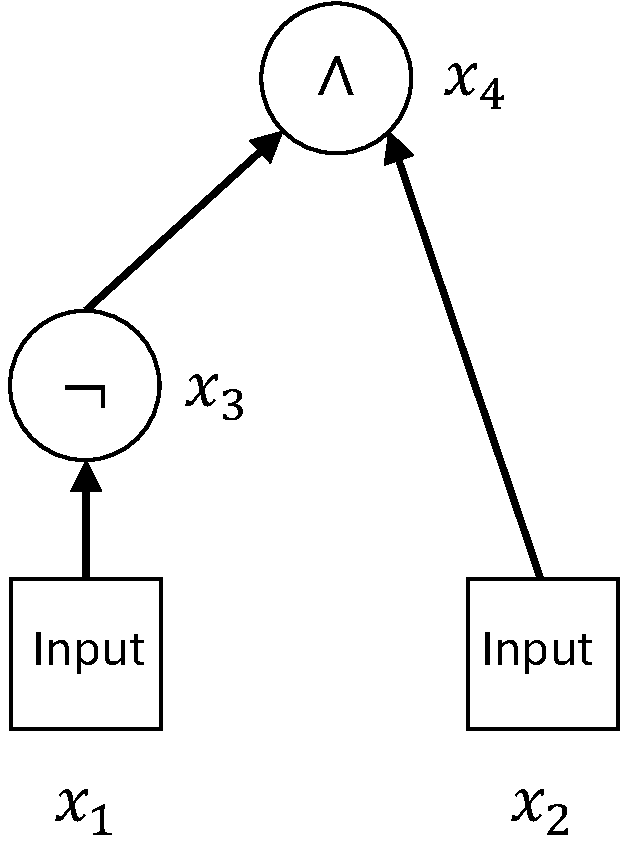
\includegraphics[width=\textwidth]{figures/circuits_2.pdf}
        \caption{Original Circuit}
        \label{subfig:original_circuit}
    \end{subfigure}
\begin{subfigure}[t]{0.54\textwidth}
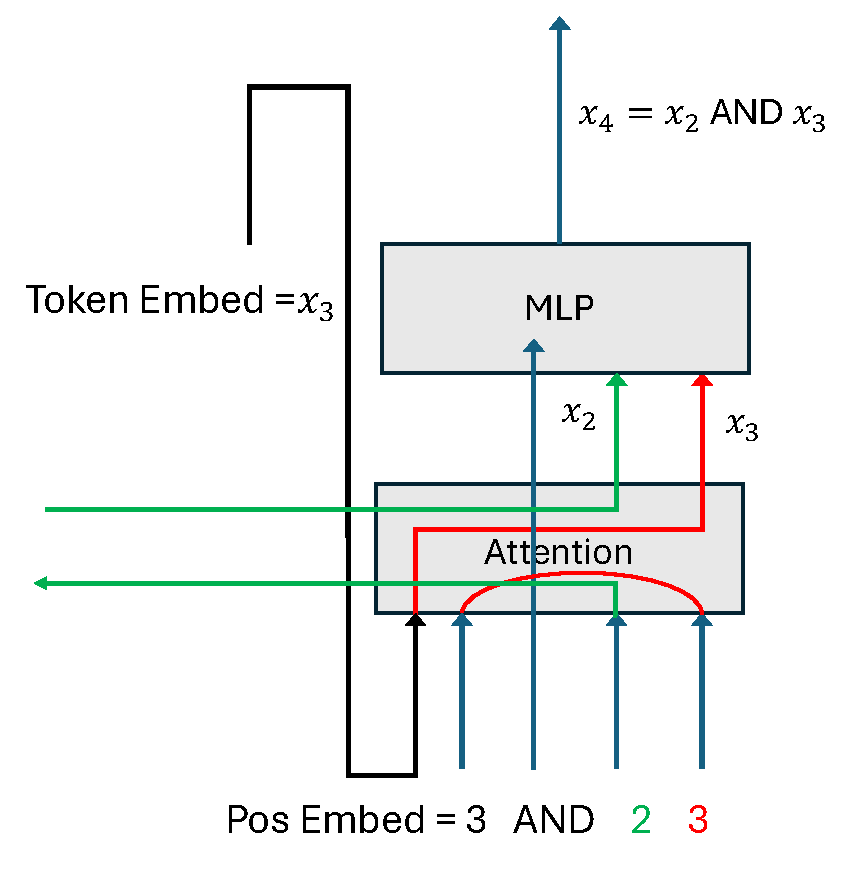
\includegraphics[width=\textwidth]{figures/cot_simulation_for_circuits.pdf}
        \caption{Forward pass of the transformer with CoT at position 3,  computing $x_4$  in \Cref{subfig:original_circuit}. The position embedding comes from the third row of the right  serialization in  \Cref{subfig:serialized_circuit}.}
        \label{subfig:cot_simulation}
    \end{subfigure}
\begin{subfigure}[b]{\textwidth}
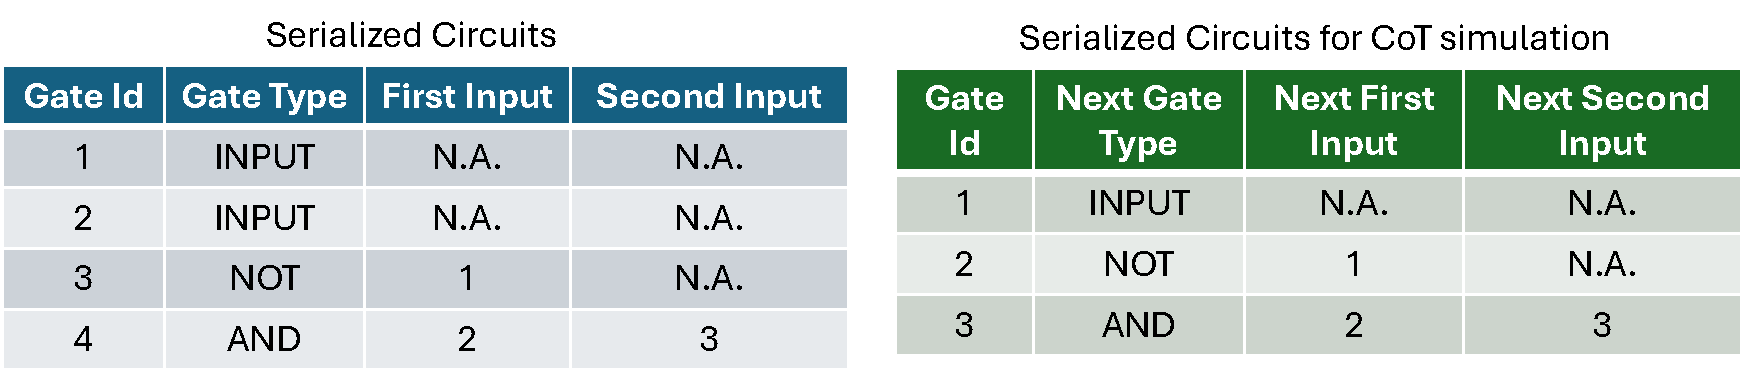
\includegraphics[width=\textwidth]{figures/serialized_circuits_row_2.pdf}
        \caption{Two ways to serialize circuits. The left (blue) one is the most natural one and the right (green) one is used to construct the position embedding so the transformer with CoT simulates the original circuit in \Cref{subfig:original_circuit}. }
        \label{subfig:serialized_circuit}
    \end{subfigure}
%\vspace{-2cm}
\caption{Illustration of \Cref{thm:cot_dlogn_main} on a 2-gate and 2-input circuit.}\label{fig:cot_simulating_circuit}
\end{center}
\vspace{-0.5cm}
\end{figure}


\begin{theorem}\label{thm:cot_dlogn_main}
For any  polynomial function $T:\mathbb{N}^+\to \mathbb{N}^+$, $\SIZE[T(n)] \subseteq \Cot[T(n)][ \log n][1]$.	In particular, $\Ppoly = \Cot[\poly(n)][ \log n][1]$.
\end{theorem}

Compared to \Cref{thm:AC0_upper_bound,thm:TC0_upper_bound}, \Cref{thm:cot_dlogn_main} shows that allowing polynomial steps of CoT strictly makes constant-depth, constant-precision, decoder-only transformer more expressive and log-precision transformers more expressive under a standard hardness assumption that $\TC^0\subsetneq \Ppoly$.\footnote{Indeed  such separation can be shown for \emph{any} polynomial steps of CoT by padding polynomially many tokens to input.}


 
\begin{proof}[Proof sketch of \Cref{thm:cot_dlogn_main}]
	The high-level proof idea is that we use each step in CoT to simulate one gate operation in the target circuit  and write the gate output as next input. To do that, we  use one position encoding to store the information for each gate, which contains four parts: the current gate id, the next gate type $\{\AND,\OR,\NOT,\True,\False\}$, and the two input gates id of the next gate. Since there are total $\poly(n)$ gates, $d(n)=\Theta(\log n)$ embedding size suffices to store the above information. The CoT here is constructed to be the values of each gate in the increasing order of id.  Therefore, in each step, we can use attention to pull the value (either computed already or it is input) of the two input gates and use a feedforward network to compute the value of the current gate. The proof idea is illustrated in \Cref{fig:cot_simulating_circuit}.
\end{proof}
 
As we can see from the proof sketch, a crucial step for CoT to simulate any depth circuit is to write the output token back to the next input position. This action resets the ``depth'' of the intermediate output in the circuit to $0$. Our theory explains the ablation experiment in \cite{wei2022chain} that when the model is prompted to output a only sequence of dots (. . .) equal to the number of tokens needed to solve the problem, the performance is no better than directly outputting the answer.


Because every regular language can be recognized by a finite state automaton (\Cref{defi:automaton}) and finite state automata can clearly be simulated by linear size circuits. The following holds as a direct corollary of \Cref{thm:cot_dlogn_main}
\begin{corollary}\label{cor:regular}
	Every regular language belongs to $\Cot[n][\log n][1]$.
\end{corollary}

Below we give a concrete regular language that constant-depth, poly-embedding-size transformers can solve only with CoT, the wording problem of permutation group over $5$ elements, $S_5$ in \Cref{thm:cot_0_n_separation}, under a standard hardness assumption that $\TC^0\subsetneq \NC^1$~\citep{yao1989circuits}.

\begin{definition}[Wording problem of group $G$]\label{defi:wording_problem}
    Given $n$ elements from $G$, $(g_1,\ldots, g_n)$, we use $\gL_G$ to denote the decision problem of whether $g_1\circ g_2\circ \cdots \circ g_n$ is equal to the identity of $G$.
\end{definition}

For convenience, in this paper, we extend the domain of $\gL_G$ to the sequence of groups encoded by binary strings. The proof of \Cref{thm:cot_0_n_separation} is a direct consequence of \Cref{thm:cot_dlogn_main,thm:TC0_upper_bound,thm:barrington}.

\begin{theorem}\label{thm:cot_0_n_separation}
   Assuming $\TC^0\subsetneq \NC^1$, the wording problem of $S_5$ , $\gL_{S_5}$ is in $\Cot[n][\log n][1]$ but not $\T[\poly(n)][ \log n]$.
\end{theorem}


\begin{theorem}[\citet{barrington1986bounded}]\label{thm:barrington}
  \!\!The wording problem of $S_5$ is $\NC^1$-complete under $\AC^0$ reductions. That is, for any decision problem $\gL$ in $\NC^1$, there is a family of $\AC^0$ circuits $\{C_n\}_{n=1}^\infty$ (constant depth, $\poly(n)$ fan-outs), such that for any $n\in\mathbb{N}^+$ and $x\in\{0,1\}^n$, $\gL(x) = \gL_{S_5}(C_n(x)).$  
\end{theorem}

 
\begin{proof}[Proof of \Cref{thm:cot_0_n_separation}]
First $\gL_{S_5}$ is a regular language, thus belonging to $\Cot[n][\log n][1]$ by \Cref{cor:regular}. Since $\gL_{S_5}$ is $\NC^1$-complete by \Cref{thm:barrington}, assuming $\TC^0\subsetneq \NC^1$,  $\gL_{S_5}$ does not belong to $\TC^0$. This proof is completed by applying \Cref{thm:TC0_upper_bound}, which says $\T[\poly(n), \log(n)]\subseteq \TC^0$. 
\end{proof}
 
\begin{figure}[t]
\begin{center}
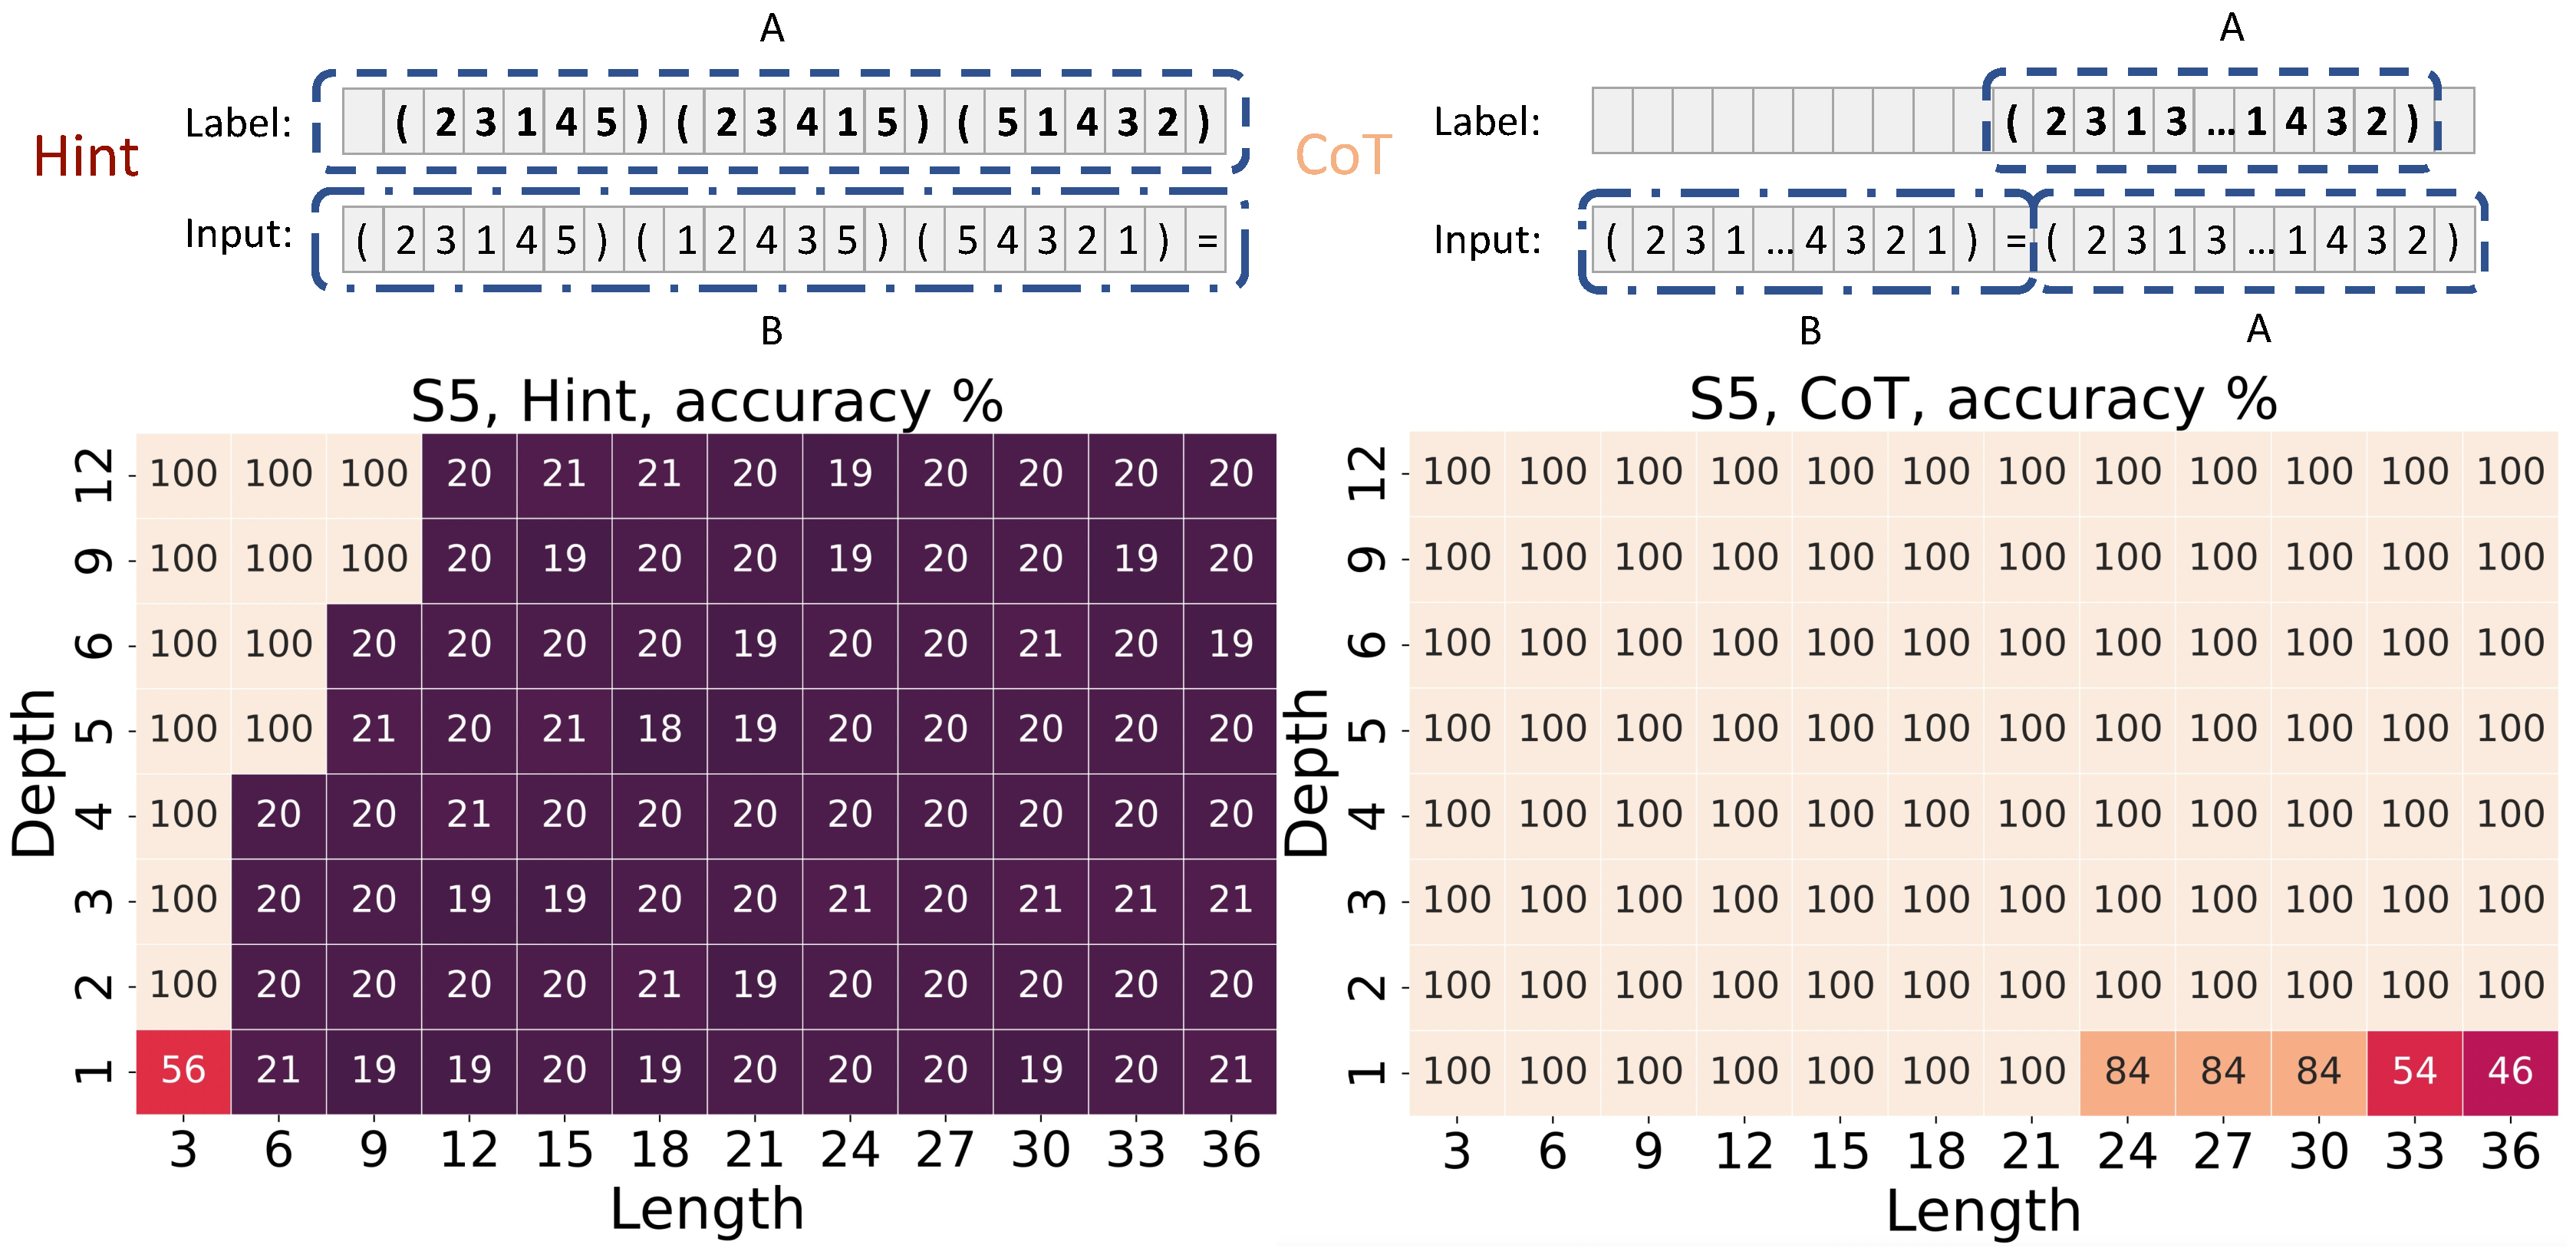
\includegraphics[width=0.96\textwidth]{figures/s5.pdf}
\caption{Permutation Composition~($S_5$). The label is the composition of all the permutations, where given two permutation $\sigma = (\sigma_1,\ldots,\sigma_5)$, $\pi = (\pi_1,\ldots,\pi_5)$, we define $\sigma\circ \pi \triangleq (\sigma_{\pi_1},\ldots, \sigma_{\pi_5})$. The chain of thoughts and hints are the partial compositions (string A). 
Only CoT can solve this task well, as predicted by our \Cref{thm:cot_0_n_separation}. Note for the most time the accuracy without CoT is $\sim20\%$, which is no better than randomly guessing a number between $1$ and $5$.
}\label{fig:s5}
\end{center}
 
\end{figure}



\paragraph{Results for $\poly(n)$ embedding size:} So far we have been focusing on the expressiveness of transformer with $O(\log n)$ embedding size, 
so it is natural to ask whether transformers can also benefit from having a larger embedding size, say $\poly(n)$? Our~\Cref{thm:cot_dpolyn_slogn_main} answers this question positively by showing that log-precision (resp. constant-precision) constant-depth poly-embedding-size decoder-only transformers with $T(n)$ steps of CoT can simulate any $T(n)$-size circuit with some $\TC^0$ (resp. $\AC^0$) oracle gates with $\poly(n)$ input. 

Formally, given a decision problem $\gL:\cup_{n=1}^\infty \{0,1\}^n\to \{0,1\}$, we use $\gL_n$ to denote the restriction of $\gL$ on $\{0,1\}^n$, which can also be viewed as an single gate with $n$ fan-ins.  We define problems that can be solved by circuits with certain sizes of gates (including oracle gates) by \Cref{defi:circuits_with_oracle}. \footnote{Our definition of complexity class solvable by circuits with oracle is slightly different from that in literature \citep{wilson1985relativized}, where the size of the oracle circuits refers to the number of wires, whereas ours refers to the number of gates.}

\begin{definition}[$\SIZE^\gL$]\label{defi:circuits_with_oracle}
	For any decision problem $\gL$ and $T(n)\subseteq O(\poly(n))$, we define $\SIZE^\gL(T(n))$ as the set of decision problems $\gL'$ such that there exists $p(n)\in \poly(n)$ and circuits $\{C_n\}_{n=1}^\infty$ where $C_n$ contains at most $O(T(n))$ $\AND$, $\OR$, $\NOT$, and $\gL_{p(n)}$ gates.
	 For a complexity class $\gC$, we define $\SIZE^{\gC}(T(n))\triangleq \cup_{\gL\in\gC}\SIZE^{\gL}(T(n))$.
\end{definition}
 

\begin{theorem}\label{thm:cot_dpolyn_slogn_main}
For any $T(n)\in\poly(n)$, it holds that $\SIZE^{\TC^0}[1+T(n)] = \Cot[T(n)][ \poly(n)][\log n]$.
Specifically, for $T(n) = 0$, we have   $\TC^0 = \SIZE^{\TC^0}[1]  = \Cot[0][ \poly(n)][\log n ] =\T[\poly(n)][\log n]$.
\end{theorem}

\begin{theorem}\label{thm:cot_dpolyn_s1_main}
For any $T(n)\in\poly(n)$, it holds that $\SIZE^{\AC^0}[1+ T(n)] = \Cot[T(n)][ \poly(n)][1]$.
Specifically, for $T(n) = 0$, we have   $\AC^0 = \SIZE^{\AC^0}[1] =\Cot[0][ \poly(n)][1] =\T[\poly(n)][1]$.
\end{theorem}


\Cref{thm:cot_dpolyn_s1_main} shows that for $T(n) = \poly(n)$ steps of CoT, using $\poly(n)$ embedding size does not improve expressiveness over using $\log(n)$ embedding size~(\Cref{thm:cot_dlogn_main}), because $\SIZE^{\TC^0}[\poly(n)] = \SIZE^{\AC^0}[\poly(n)] = \SIZE[\poly(n)]$. However,  \Cref{thm:transformer_polyn_stronger_than_logn} shows that for any specific polynomial $T(n)=n^k$ steps of CoT, increasing embedding width from $O(\log (n))$ to $\poly(n)$  make transformers strictly more powerful. 

\begin{theorem}\label{thm:transformer_polyn_stronger_than_logn}
	For any $s(n) = O(\log n)$, $\T[\log n][s(n)]\subsetneq \T[\poly(n)][s(n)]$ and for all $ k\in\mathbb{N}$, $\Cot[n^k][ \log n][s(n)]\subsetneq \Cot[n^k][\poly(n)][s(n)]$. 
\end{theorem}

%We also remark that \Cref{thm:cot_dpolyn_slogn_main,thm:cot_dpolyn_s1_main} implies that
%\textbf{logarithmically many CoT steps does not solve inherently serial problems.} Formally, we have the following theorem:
%
%\begin{theorem}\label{thm:cot_logn_dpolyn_constant_depth}
% $\AC^0 = \Cot[\log n][ \poly(n)][1]$ and  $\TC^0 = \Cot[\log n][ \poly(n)][\log n]$.
%\end{theorem}
%
%\Cref{thm:cot_logn_dpolyn_constant_depth} holds because $\SIZE^{\AC^0}[\log n] = \AC^0$ and $\SIZE^{\TC^0}[\log n] = \TC^0$. This is because one can always write any circuit $C\in \SIZE^{\AC^0}[T(n)]$ circuits as an $\OR$ of $2^{T(n)}$ disjoint subcircuits, where each of them enumerates all possible values of $T(n)$ gates in $C$ and output the value of the last gate in this possibility if all the intermediate gate values are consistent, otherwise, it outputs $0$. This enumeration can be done in parallel and thus only takes constant depth. When $T(n)=O(\log n)$, this only leads $\poly(n)$ factor of explosion in circuit size and thus still in $\TC^0$. Same argument holds for $\AC^0$ as well.
